\documentclass[12pt, a4paper]{article}
\usepackage{geometry}
\geometry{verbose,tmargin=2cm,bmargin=2cm,lmargin=3cm,rmargin=3cm}
\usepackage{verbatim}
\usepackage[normalem]{ulem}
\usepackage{colortbl}
\usepackage{graphicx}
\usepackage{algorithm,algpseudocode}
\usepackage[colorlinks,citecolor=red,urlcolor=blue,bookmarks=false,hypertexnames=true]{hyperref}
\usepackage{url}

\makeatother
\date{}
\begin{document}

\title{\Large 16-833: Robot Localization and Mapping, Spring 2024\\
	\textbf{Homework 2 - SLAM using Extended Kalman Filter (EKF-SLAM)}}
\maketitle
\begin{flushright}
	\textbf{\uline{Due: Friday March 15, 11:59pm, 2024}}
	\par\end{flushright}


Your homework should be submitted as a\textbf{ typeset PDF file} along
with a\textbf{ }folder\textbf{ }including\textbf{ code} \textbf{only(no data)}.
The PDF and code must be submitted on \textbf{Gradescope}.
In your implementation, please only fill in the functions marked by $\mathtt{TODO}$,
and play with parameters, and keep other parts unchanged.
If you have questions, post them on Piazza or come to office hours.
Please do not post solutions or codes on Piazza.

This homework must be done \textbf{individually}, and plagiarism will
be taken seriously. You are free to discuss and troubleshoot with
others, but the code and writeup must be your own. Note that you should
list the name and Andrew ID of each student you have discussed with
on the first page of your PDF file.

\section{Theory (40 points)}

In this part we are going to guide you through some steps of EKF-SLAM
in math. This will be helpful in your implementation in the next problem.

A robot is moving on the 2D ground plane. In each time step $t$,
the robot is controlled to move forward (the $x$-direction of the
robot's coordinates) $d_{t}$ meters, and then rotate $\alpha_{t}$
radian. The pose of the robot in the global coordinates at time $t$
is written as a vector $\mathbf{p}_{t}=\left[\begin{array}{ccc}
			x_{t} & y_{t} & \theta_{t}\end{array}\right]^{\top}$, where $x_{t}$ and $y_{t}$ are the 2D coordinates of the robot's
position, and $\theta_{t}$ is the robot's orientation.

\begin{enumerate}
	\item Based on the assumption that there is no noise or error in the
	      control system, predict the next pose $\mathbf{p}_{t+1}$ as a nonlinear
	      function of the current pose $\mathbf{p}_{t}$ and the control inputs
	      $d_{t}$ and $\alpha_{t}$. (5 points)

	\item However, in reality there are some errors when the robot moves
	      due to the mechanism and the terrain. Assume the errors follow Gaussian
	      distributions: $e_{x}\sim\mathcal{N}\left(0,\sigma_{x}^{2}\right)$
	      in $x$-direction, $e_{y}\sim\mathcal{N}\left(0,\sigma_{y}^{2}\right)$
	      in $y$-direction, and $e_{\alpha}\sim\mathcal{N}\left(0,\sigma_{\alpha}^{2}\right)$
	      in rotation respectively (all in robot's coordinates). For details, please see Fig.~\ref{fig:1b}.
	      Now if the uncertainty of the robot's pose at time $t$ can be represented as
	      a 3-dimensional Gaussian distribution $\mathcal{N}\left(0,\Sigma_{t}\right)$,
	      what is the predicted uncertainty of the robot at time $t+1$? Please
	      express it as a Gaussian distribution with zero mean. (5 points)
	      \begin{figure}
		      \centering
		      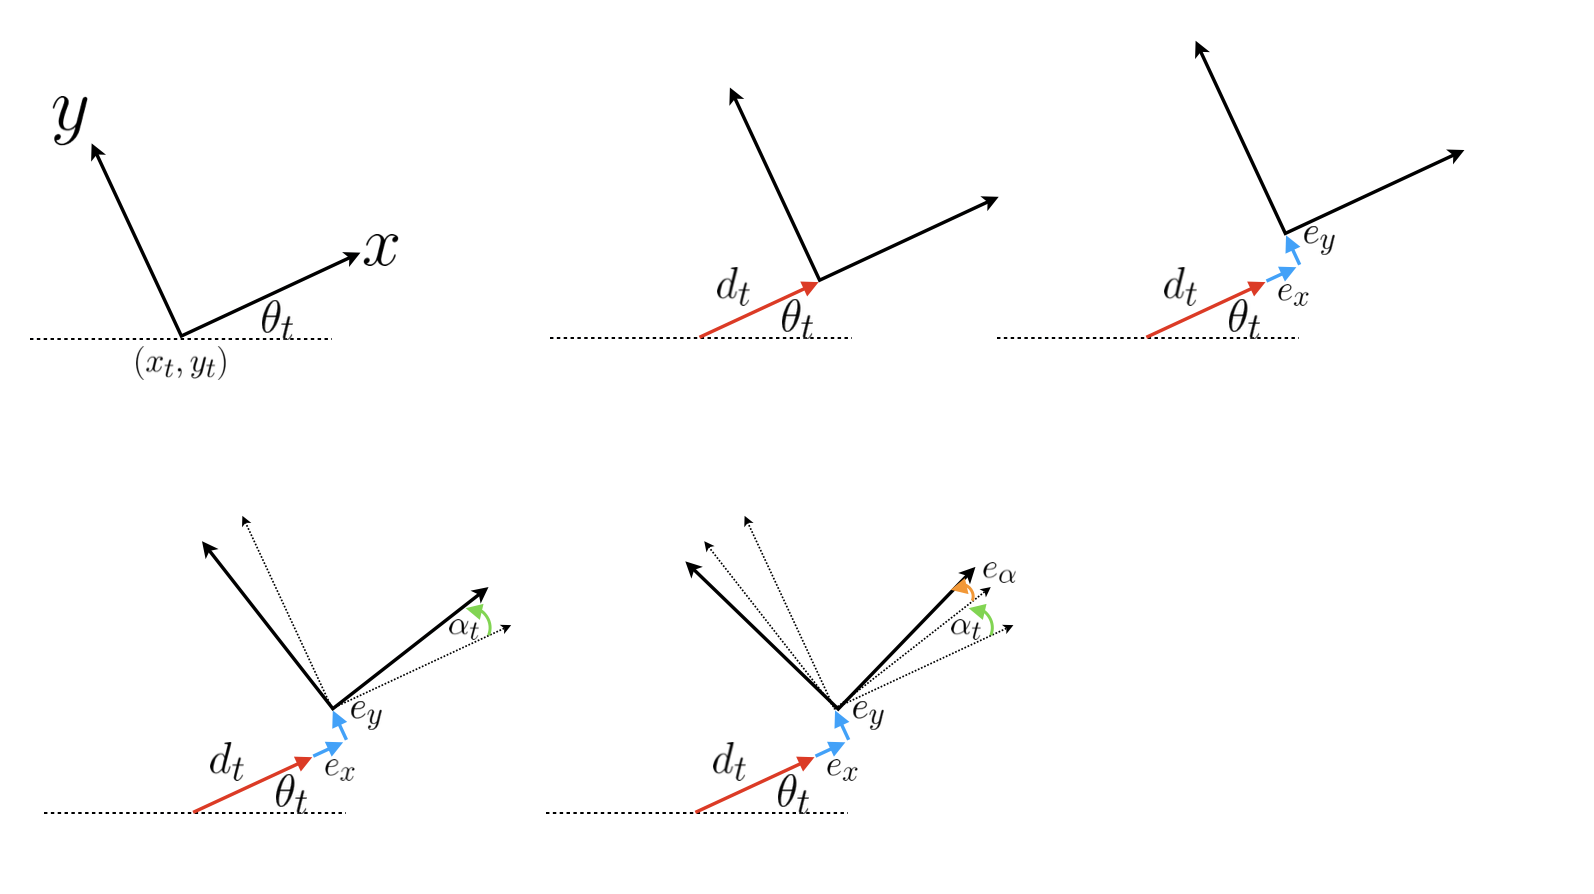
\includegraphics[width=0.99\textwidth]{1b.png}
		      \caption{0) Robot state; 1) robot moves $d_t$ along its x-axis;
			      2) due to noise it shifted $e_x$ and $e_y$ along its x and y axises respectively;
			      3) robot rotates $\alpha_t$ after shifting;
			      4) due to noise the rotation is disturbed by $e_\alpha$.}
		      \label{fig:1b}
	      \end{figure}

	\item Consider a landmark $l$ being observed by the robot at time $t$
	      with a laser sensor which gives a measurement of the bearing angle
	      $\beta$ (in the interval $(-\pi,\pi]$) and the range $r$, with
	      noise $n_{\beta}\sim\mathcal{N}\left(0,\sigma_{\beta}^{2}\right)$
	      and $n_{r}\sim\mathcal{N}\left(0,\sigma_{r}^{2}\right)$ respectively.
	      Write down the estimated position $\left(l_{x},l_{y}\right)$ of landmark
	      $l$ in global coordinates as a function of $\mathbf{p}_{t}$, $\beta$,
	      $r$, and the noise terms. (5 points)

	\item According to 1.3, if we now know that $l$ is at $\left(l_{x},l_{y}\right)$
	      in the global coordinates, please predict the measurement of bearing
	      and range based on $l_{x}$, $l_{y}$, $\mathbf{p}_{t}$, and the
	      noise terms (use functions $\mathit{np.arctan2}(.)$ and $\mathit{warp2pi}(.)$
	      that warps an arbitrary angular value into the range $(-\pi,\pi]$
	      if needed). (5 points)

	\item An important step in EKF-SLAM is to find the measurement Jacobian
	      $H_{p}$ with respect to the robot pose. Please apply the results
	      in 1.4 to derive the analytical form of $H_{p}$ (Note: $H_{p}$ should
	      be a $2\times3$ matrix represented by $\mathbf{p}_{t}$ and $l$).
	      (10 points)

	\item For each measurement of bearing and range, we also need a measurement
	      Jacobian $H_{l}$ with respect to its corresponding landmark $l$.
	      Please again derive the analytical form of $H_{l}$ (Note: $H_{l}$
	      should be a $2\times2$ matrix represented by $\mathbf{p}_{t}$ and
	      $l$). Why do we not need to calculate the measurement Jacobian with
	      respect to other landmarks except for itself (Hint: based on what
	      assumption)? (10 points)
\end{enumerate}

Note in this section, in addition to conventional linearization with additive noise (in the form of $x_{t+1} = g(x_t, u_t) + \epsilon_t$), you may encounter non-additive noise (in the form of $x_{t+1} = g(x_t, u_t, \epsilon_t))$. \href{https://en.wikipedia.org/wiki/Extended_Kalman_filter#Non-additive_noise_formulation_and_equations}{Derivation of the linearization} for this formulation can be helpful.
Also, all the noise reading ($\epsilon, n$) can be regarded as infinitismal. Second and higher order terms comprised by their products can be ignored.

\section{Implementation and Evaluation (45 points)}

In this part you will implement your own 2D EKF-SLAM solver in Python.
The robot in problem 1 starts with observing the surrounding environment
and measuring some landmarks, then executes a control input to move.
The measurement and control steps are repeated several times. For
simplicity, we assume the robot observes the same set of landmarks
in the same order at each pose. We want to use EKF-SLAM to recover
the trajectory of the robot and the positions of the landmarks from
the control input and measurements.

\begin{enumerate}
	\item Find the data file $\mathtt{data/data.txt}$ that contains the
	      control inputs and measurements. Open the file to take a look. The
	      data is in the format of measurements$=\left[\begin{array}{ccccc}
				      \beta_{1} & r_{1} & \beta_{2} & r_{2} & \cdots\end{array}\right]$, where $\beta_{i}$, $r_{i}$ correspond to landmark $l_{i}$, and control$=\left[\begin{array}{cc}
				      d & \alpha\end{array}\right]$ (refer to problem 1 for the notations). The
	      lines are in sequential time order.

	      What is the fixed number
	      of landmarks being observed over the entire sequence? (5 points)

	\item The $\mathtt{code/}$ folder contains the Python code file
	      $\mathtt{ekf\_slam.py}$. Follow the comments and fill in the functions $\mathtt{warp2pi},~\mathtt{init\_landmarks}, ~\mathtt{predict}, ~\mathtt{update}$ to enable the system. The visualization will show the trajectory and the landmarks with their covariances in the shape of 3-$\sigma$ ellises. It will be updated sequentially, and you may process the next step by clicking your mouse or hitting any key.

	      Attach a clear figure of your
	      visualization in the write up once all the steps are finished. (25 points)

	\item In the output figure, the magenta and blue ellipses represent
	      the predicted and updated uncertainties of the robot's position (orientation
	      not shown here) at each time respectively. Also, the red and green
	      ellipses represent the initial and all the updated uncertainties of
	      the landmarks, respectively.

	      Describe how EKF-SLAM improves the estimation
	      of both the trajectory and the map by comparing the uncertainty ellipses.
	      (5 points)

	\item Now let's evaluate our output map. Suppose we have the ground
	      truth positions of all the landmarks:

	      $\left[\begin{array}{cccc}
				      l_{1}^{\top} & l_{2}^{\top} & \cdots & l_{k}^{\top}\end{array}\right]=\left[\begin{array}{cccccccccccc}
				      3 & 6 & 3 & 12 & 7 & 8 & 7 & 14 & 11 & 6 & 11 & 12\end{array}\right]$.

	      Plot the ground truth positions of the landmarks in the output figure
	      (code already provided in function $\mathtt{evaluate}$)
	      and attach it below. Is each of them inside the smallest corresponding
	      ellipse? What does that mean?

	      Compute and report the \emph{Euclidean} and
	      \emph{Mahalanobis} distances of each landmark estimation with respect
	      to the ground truth. What do the numbers tell you? (10 points)
\end{enumerate}

\section{Discussion (15 points)}

\begin{enumerate}
	\item Explain why the zero terms in the initial landmark covariance
	      matrix become non-zero in the final state covariance matrix (print
	      out the final $P$ matrix to check it). Additionally, when setting
	      the initial value for the full covariance matrix $P$ (line 201 in
	      $\mathtt{ekf\_slam.py}$) an assumption is made regarding certain cross-covariances
	      that is not necessarily correct. Can you point out what that is? (5
	      points)

	\item Play with the parameters (line 163-167). Modify each parameter~$\sigma_{x}$,
	      $\sigma_{y}$, $\sigma_{\alpha}$$\sigma_{b}$, $\sigma_{r}$ at a
	      time and fix the others. In particular, you should set each parameter
	      to be 10 times larger/smaller to the original parameters to discuss
	      how each parameters influence the results. Attach figures for
	      better explanation. (10 points)


	\item With the same set of landmarks being observed all the time, the
	      EKF-SLAM system runs in constant time in each iteration. However,
	      for real-world problems, the total number of landmarks can grow unbounded
	      if the robot keeps exploring new environments. This will slow down
	      the EKF-SLAM system a lot and become a crucial problem for real-time
	      applications. What changes can we make to the EKF-SLAM framework to
	      achieve constant computation time in each cycle or at least speed
	      up the process (list as many possible solutions as you can think of)?
	      (Bonus 5 points)
\end{enumerate}

\section{Code Submission}

Upload your $\mathtt{ekf\_slam.py}$.
Please do not upload the $\mathtt{data/}$ folder or any other data
or image.
\end{document}

